% ----------------------------------------------------------
\section{Monitoramento de baixo custo da qualidade do ar}\label{section:low-cost-air-quality-monit}
% ----------------------------------------------------------

Segundo Emily Snyder e colaboradores  o monitoramento da qualidade do ar tem experimentado uma mudança de paradigma na forma como os dados são coletados \cite{Snyder2013}. Os avanços recentes em instrumentação eletrônica unido a necessidade de soluções alternativas que complementem as técnicas de monitoramento tradicionais, têm contribuído para um crescente interesse no desenvolvimento de sensores de qualidade do ar de baixo custo \cite{Kumar2015,Lewis2018Low-costApplications}. Esses novos sensores possuem características essenciais como tamanho e peso reduzidos, baixo consumo de potência, baixo custo e facilidade de uso, que os colocam em vantagem com relação aos instrumentos de referência, e que têm criado as condições para aprimorar uma série de aplicações de monitoramento e gerar novas \cite{Snyder2013,Lewis2018Low-costApplications}.

Este tipo de tecnologia possibilitaria a agências públicas, entidades reguladoras e de pesquisa utilizar um maior volume de sistemas de monitoramento, e assim diversificar e complementar as aplicações de monitoramento para fins de pesquisa e regulamentação e validar modelos atmosféricos \cite{Lewis2018Low-costApplications}. Estes sistemas podem prover informação temporal qualitativa relevante sobre o nível de poluição atmosférica em uma determinada localidade por períodos de dias a meses \cite{Castell2018LocalizedNodes}, como por exemplo, os momentos do dia em que a poluição é maior ou menor \cite{Zimmerman2018AMonitoring}, ou observar a sua variação ao longo do tempo \cite{Castell2017CanEstimates}. Igualmente, os sistemas de baixo custo têm sido utilizados para detectar de áreas com níveis de concentração elevados nas cidades \cite{Mead2013TheNetworks} e elaborar mapas de poluição \cite{Huang2019EstimatingMeasurements}.

Para Emily Snyder e colaboradores o uso deste tipo de sensores pode levar a uma melhor proteção da saúde pública e do meio ambiente \cite{Snyder2013}. Sensores de baixo custo podem ser usados para prover informação representativa de exposição pessoal a poluentes, com elevada resolução temporal \cite{Mead2013TheNetworks,Jerrett2017ValidatingScience}. Igualmente, esta nova forma de medição, por ser de baixo custo e de fácil operação, pode ser instalada em comunidades \cite{Mahajan2020APollution}, escolas e áreas residenciais \cite{Castell2018LocalizedNodes}, provendo informação à população sobre a qualidade do ar que respiram, e colocando os processos de monitoramento e medição nas mãos de comunidades e indivíduos \cite{Lewis2018Low-costApplications}.

% ----------------------------------------------------------
\subsection{Princípios de funcionamento dos sensores de gases de baixo custo}
% ----------------------------------------------------------

Segundo seu princípio de funcionamento, os sensores de baixo custo utilizados para a medição de poluentes na atmosfera podem ser classificados em: sensores de material particulado e sensores de gases \cite{Maag2018ADeployments}. Os sensores de material particulado funcionam baseados em princípios  de detecção óticos que medem o espalhamento ou a adsorção da luz pelas partículas \cite{Rai2017End-userMonitoring}. Já os sensores de gases podem ser subdivididos em duas classes: os óticos e os que dependem da interação entre o material transdutor e o composto gasoso \cite{Snyder2013}.
	
O princípio ótico de medição consiste em expor o composto gasoso a um feixe de luz, com determinado comprimento de onda, e medir o efeito dessa interação com um detector fotossensível \cite{Rai2017End-userMonitoring}. Dentro desse grupo, os sensores mais comuns são os infravermelhos não-dispersivos (\gls{ndir}, por suas siglas em inglês), usados para medir \acrshort{co2} e \acrshort{ch4}, e os detectores de foto-ionização (\gls{pid}, por suas siglas em inglês) que utilizam luz ultravioleta e são usados para medir compostos orgânicos voláteis \cite{Snyder2013}.

Dentre os sensores de gases que operam a partir da interação entre o material transdutor e o composto gasoso, os mais populares são: os semicondutores de óxido metálico (\gls{mos}, por suas siglas em inglês) e os de princípio eletroquímico (\gls{ec}, por suas siglas em inglês). Esses são os sensores mais comumente utilizados para medir gases tóxicos como \acrshort{co}, \acrshort{nox}, \acrshort{o3} e \acrshort{so2} \cite{Lewis2018Low-costApplications}.

Os sensores \gls{ec}, em comparação com os \gls{mos}, costumam ter um menor consumo de potência, maior seletividade, menores limites de detecção e uma relação linear com a concentração. Os sensores \gls{mos}, por sua parte, têm custos menores e seu condicionamento eletrônico costuma ser mais simples \cite{Rai2017End-userMonitoring}. Neste trabalho serão abordados apenas os sensores eletroquímicos por serem os mais utilizados para o monitoramento de baixo custo da qualidade do ar e pela relação linear entre suas respostas e a concentração de gás.

É importante ressaltar que o atual estado da arte dos sensores de baixo custo impossibilita que eles substituam os métodos de medição de referência. Contudo, resultados promissores têm sido encontrados em várias áreas, principalmente naquelas em que as técnicas convencionais não poderiam ser implementadas devido a limitações como a pouca portabilidade, o elevado consumo energético e o custo.

% ----------------------------------------------------------
\subsection{Iniciativas de monitoramento de baixo custo da qualidade do ar}
% ----------------------------------------------------------

Diversas iniciativas de monitoramento têm implementado e disponibilizado recursos para a coleta e o acesso a dados de redes de monitoramento da qualidade do ar compostas por sensores de gases de baixo custo. Fabricantes como AQMesh, Vaisala, i-Blades, Libelium e Clarity fornecem, junto com os equipamentos de monitoramento, serviços de visualização e de análise de dados, que são oferecidos como Software como Serviço (SaaS), Plataforma como Serviço (PaaS) ou Sensoriamento como Serviço. Os custos destes equipamentos oscila entre 1.000,00 - 10.000,00 EUR, sem incluir custos de operação, e o acesso aos dados dos sensores está condicionado a subscrições nos serviços de nuvem providos pelos próprios fabricantes \cite{Karagulian2019ReviewMonitoring}. Destes, apenas a Clarity fornece um mapa aberto para visualização geo-localizada e das séries históricas das leituras dos sensores instalados pelo globo. Com relação à propriedade intelectual, a exceção da Libelium, os equipamentos dos outros fabricantes mencionados encontram-se na categoria de "caixa preta". 

Outras iniciativas, lideradas por comunidades e instituições de investigação, fornecem recursos para o acesso aberto aos dados e alguns deles incluem também código e \textit{hardware} aberto. Alguns delas são o \textit{Habitat Map} \cite{HabitatMap2023AirCasting}, \textit{IQAir} \cite{IQAir2023}, \textit{Air Quality Egg Portal} \cite{AirQualityEgg2023AirPortal}, o projeto \textit{Sensor.Community} \cite{Sensor.Community2023LuftMap}, PurpleAir \cite{PurpleAir2023PurpleAirMonitoring}, \textit{Smart Citizen} \cite{SmartCitizen2023SmartCitizen}, e o mapa da rede \textit{uRADMonitor} \cite{uRADMonitor2023PM2.5URADMonitor}. O custo de aquisição das plataformas de sensores destas iniciativas varia entre 60,00 – 3.750,00 USD. A maior parte das iniciativas comunitárias disponibilizam os dados e o acesso à plataforma \textit{web} de monitoramento de forma gratuita, mas é necessário adquirir um sensor para se conectar à rede.

\textit{Habitat Map} disponibiliza seu sensor \textit{AirBeam} por 249.00 USD. \textit{AirBeam} mede material particulado, temperatura e umidade relativa, possui pequenas dimensões, peso reduzido e é portátil \cite{HabitatMap2023AirCasting}. O acesso aos dados dos monitores ativos estão acessíveis de forma aberta e gratuita na plataforma \textit{HabitatMap}, mas o registro de sensores nela está condicionado à compra de sensores \textit{AirBeam}. As informações sobre a fabricação do sensor e da \acrshort{api} de monitoramento não estão acessíveis publicamente. O \textit{HabitatMap} disponibiliza também medições de sensores \textit{PurpleAir} e de estações de referência. A Figura \ref{fig:habitat-map-initiative} ilustra o sensor e o painel principal de \textit{HabitatMap}.

\begin{figure}[h]
    \centering
    \caption{A iniciativa \textit{Habitat Map} e o sensor \textit{AirBeam}}
    \begin{subfigure}{0.44\textwidth}
        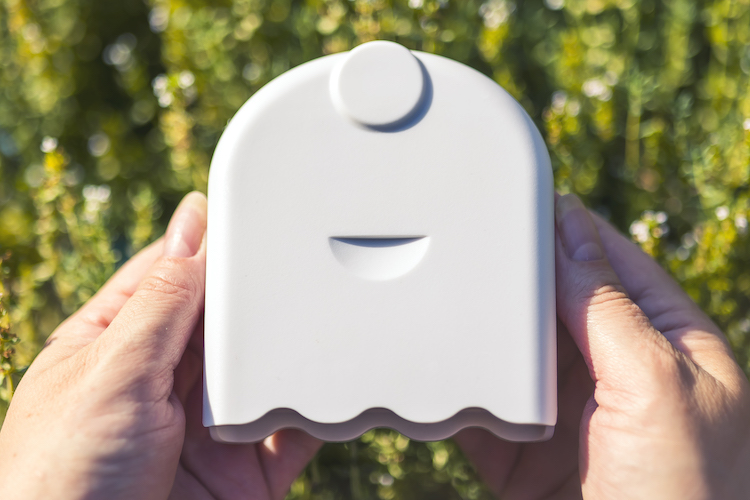
\includegraphics[width=\textwidth]{chapters/1-MONITORAMENTO/Figuras/airbeam-buy-it-now.jpg}
        \caption{O sensor \textit{AirBeam}}
        \label{fig:air-beam}
    \end{subfigure}
    \hfill
    \begin{subfigure}{0.54\textwidth}
        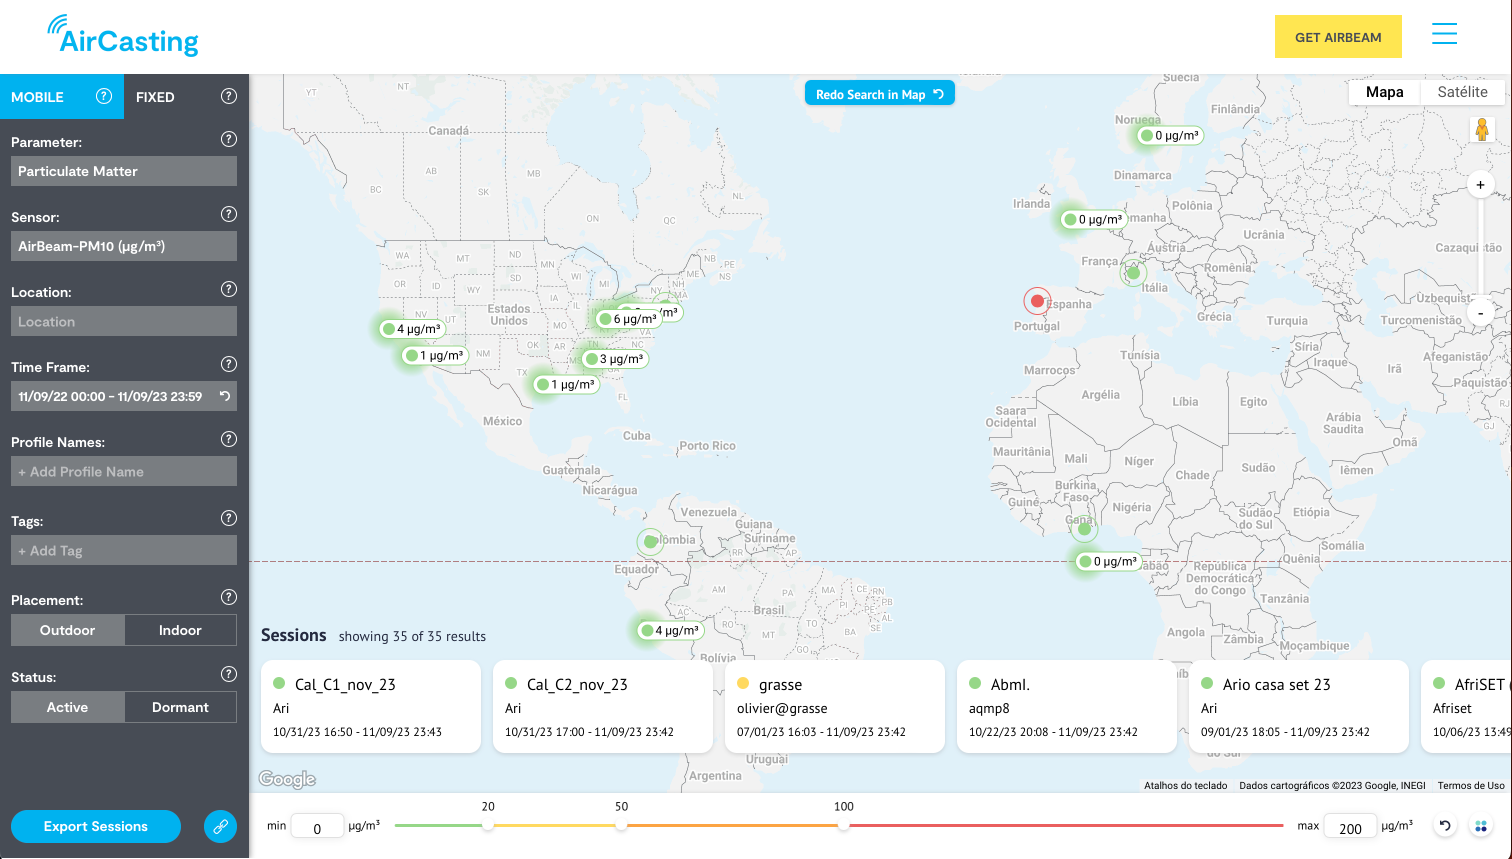
\includegraphics[width=\textwidth]{chapters/1-MONITORAMENTO/Figuras/Habitat Map.png}
        \caption{Painel principal da plataforma \textit{web} \textit{HabitatMap}}
        \label{fig:habitat-map}
    \end{subfigure}
    \hfill
    \label{fig:habitat-map-initiative}
    \fonte{\cite{HabitatMap2023AirCasting}}
\end{figure}

\textit{Air Quality Egg} é uma plataforma de monitoramento de baixo custo com foco no ensino básico e fundamental para abordar temas sobre qualidade do ar, poluição atmosférica e ciência cidadã. Assim como \textit{HabitatMap} os dados de monitoramento estão acessíveis mas para o registro de dados deve ser feito por meio de um dos seus sensores, chamados de \textit{Egg}. É possível adquirir diferentes modelos de \textit{Egg} que medem temperatura, umidade relativa, pressão atmosférica, \acrshort{co2}, \acrshort{so2}, \acrshort{no2}, \acrshort{mp}, \acrshort{o3}, \acrshort{co}, \acrshort{voc} e \acrshort{h2s}. Os modelos também podem incluir módulo \acrshort{gps} e bateria. Dependendo da configuração de sensor escolhida os valores podem oscilar desde 650.00 USD até 1485.00 USD. Além disso, para acessar outros recursos da plataforma é necessária uma subscrição, que é gratuita para indivíduos mas tem um custo adicional de 2000.00 USD para organizações.

\begin{figure}[h]
    \centering
    \caption{O portal \textit{Air Quality Egg} e o sensor \textit{Egg}}
    \begin{subfigure}{0.49\textwidth}
        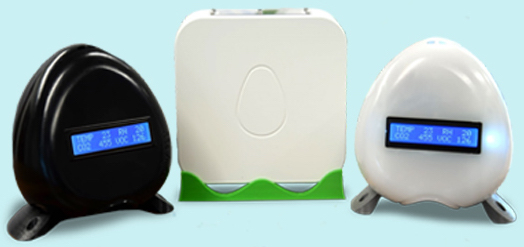
\includegraphics[width=\textwidth]{chapters/1-MONITORAMENTO/Figuras/Air Quality Egg.jpg}
        \caption{O sensor \textit{Egg}}
        \label{fig:air-quality-egg}
    \end{subfigure}
    \hfill
    \begin{subfigure}{0.49\textwidth}
        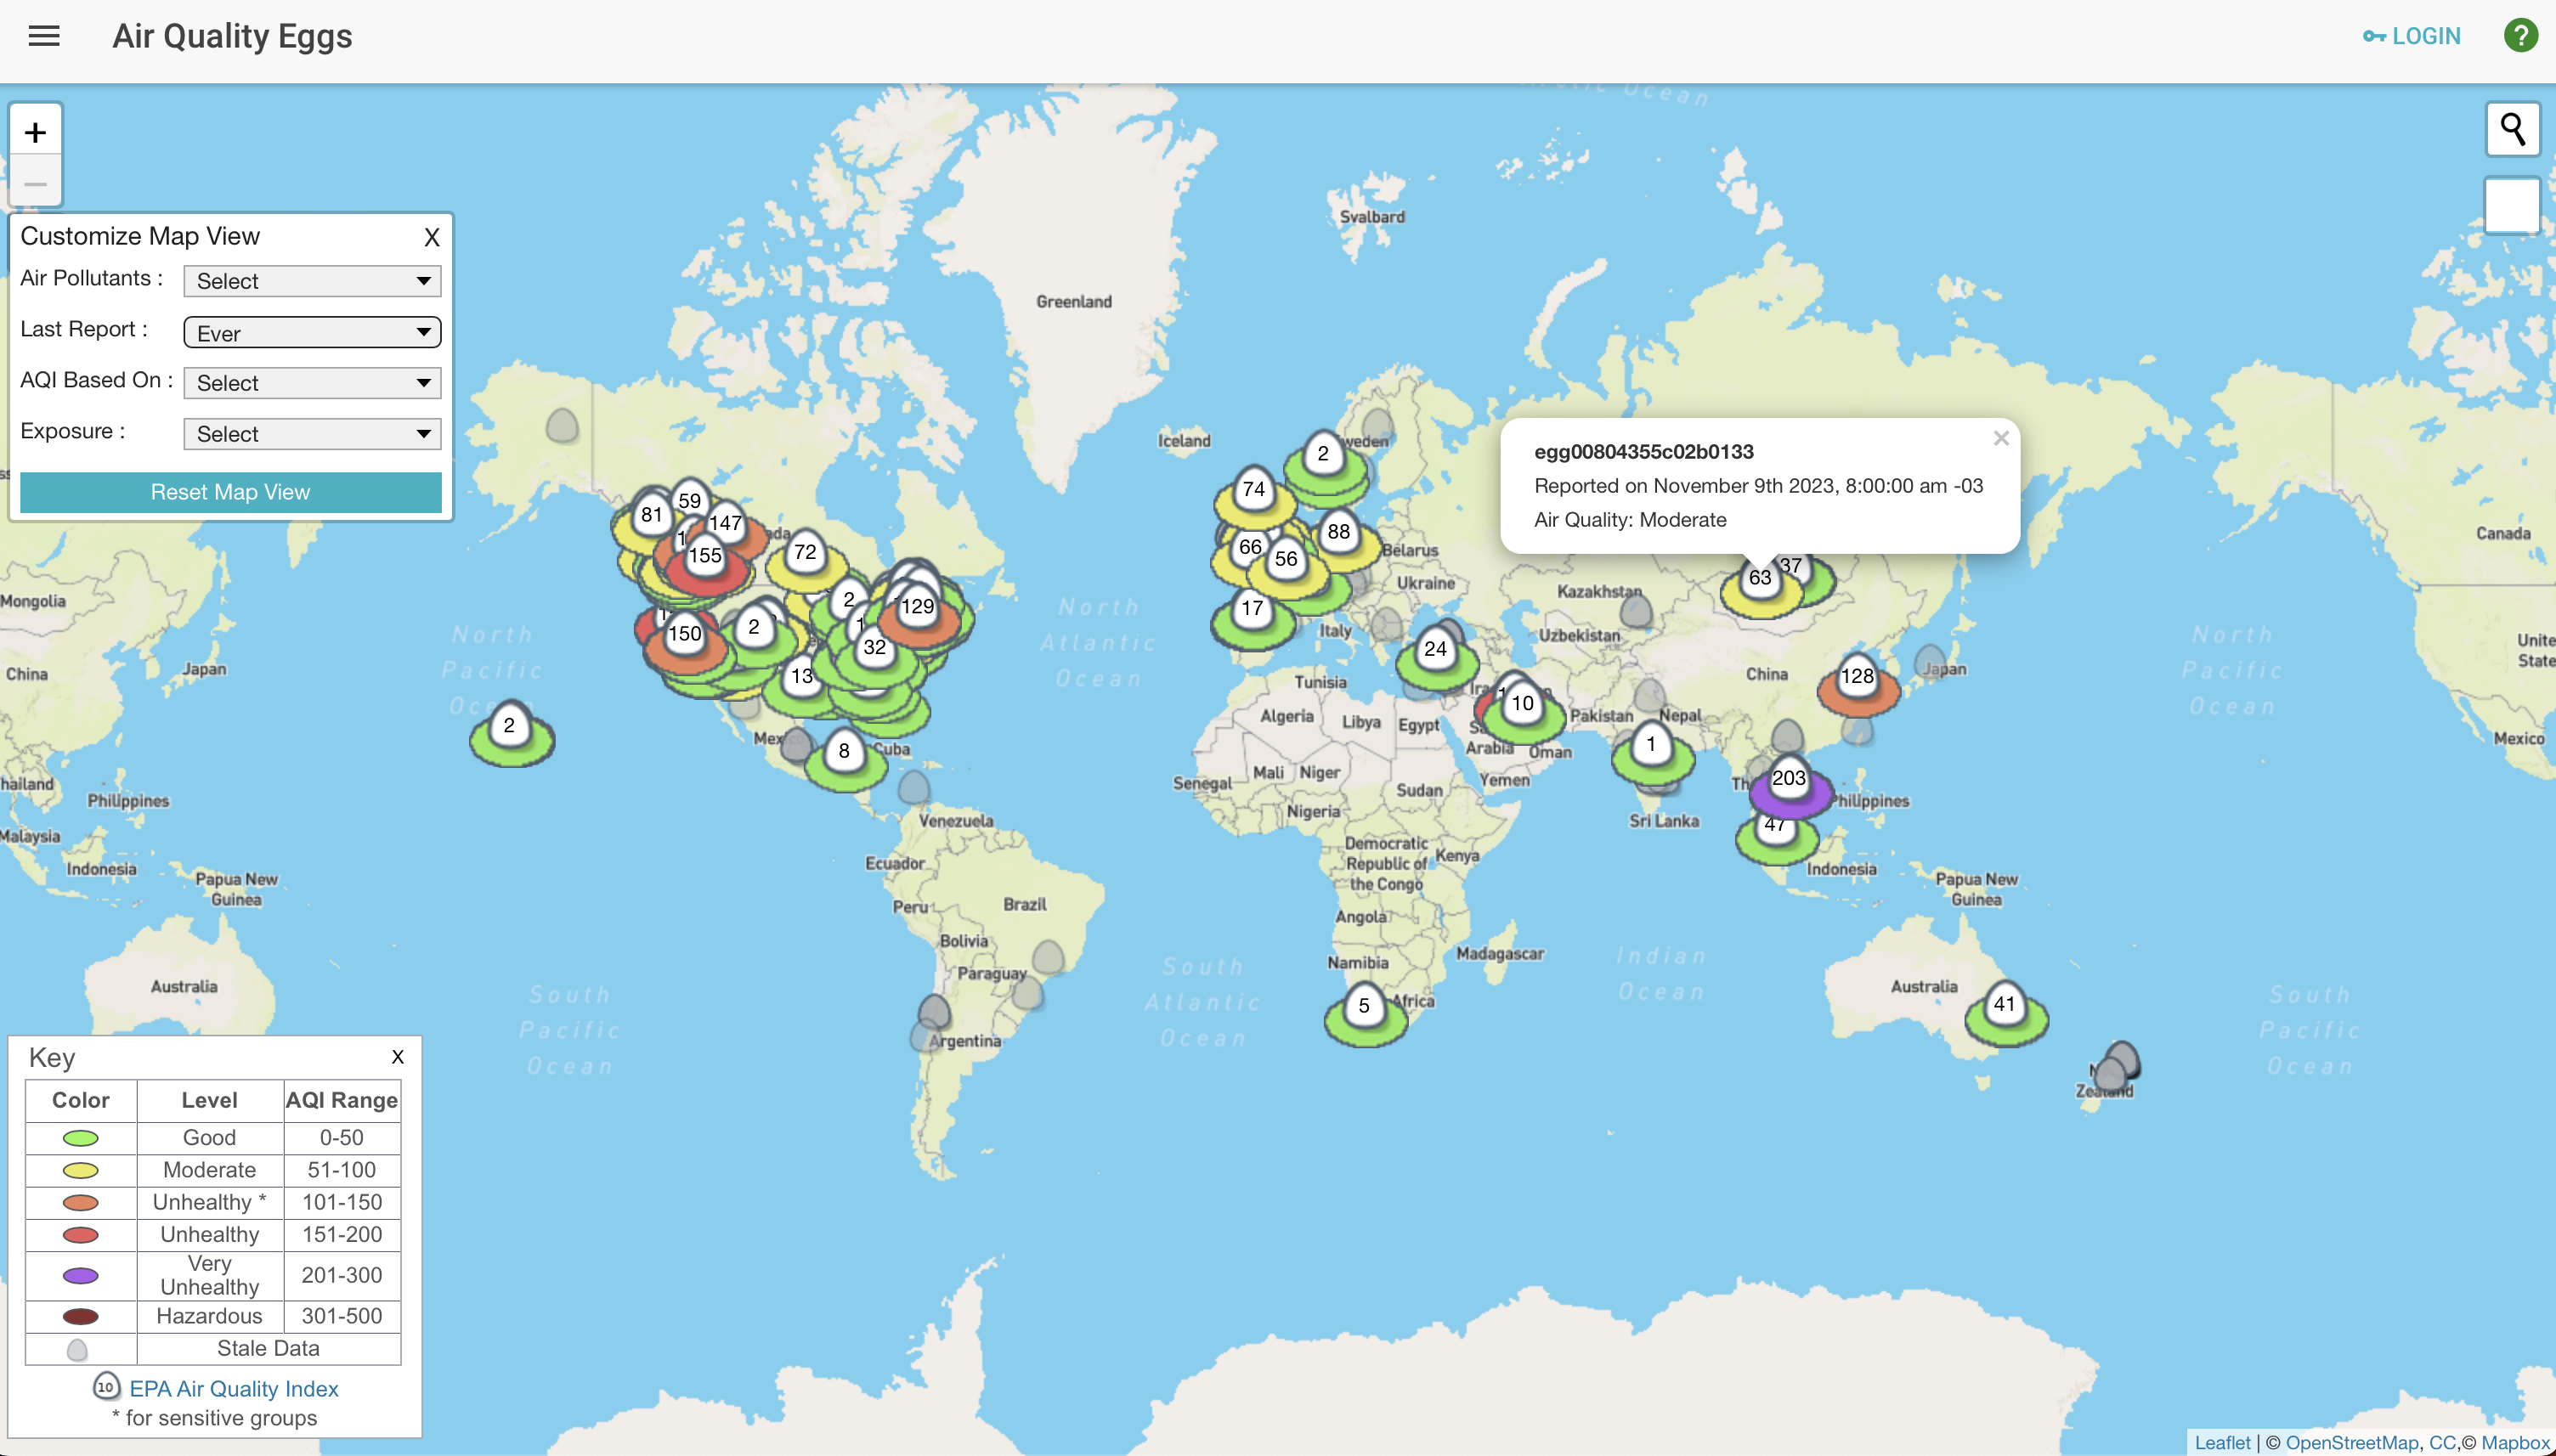
\includegraphics[width=\textwidth]{chapters/1-MONITORAMENTO/Figuras/Air Quality Egg Portal.png}
        \caption{Painel principal da plataforma \textit{web} \textit{Air Quality Egg}}
        \label{fig:air-quality-egg-portal}
    \end{subfigure}
    \hfill
    \label{fig:air-quality-egg-initiative}
    \fonte{\cite{AirQualityEgg2023AirPortal}}
\end{figure}

\textit{uRADMonitor}, \textit{IQAir} e \textit{PurpleAir} possuem modelos de negócio semelhantes aos mencionados acima, no sentido de ser necessário adquirir um sensor para registar dados nas plataformas. O que os diferencia, contudo, é que disponibilizam mais de um modelo de sensor assim como acesso aos dados e serviços de software através de \acrshort{api}s. \textit{uRADMonitor} vende 12 modelos de monitores da qualidade do ar com preços que vão desde 200.00 uSD até 3750.00 USD dependendo da quantidade de gases que medem, a aplicação e precisão. Os sensores utilizados por \textit{uRADMonitor} são diversos e podem medir \acrshort{mp}, \acrshort{co}, \acrshort{so2}, \acrshort{o3}, \acrshort{no2}, formaldeído, \acrshort{voc}, \acrshort{nh3}, radiação e outros gases tóxicos. Não existe um custo adicional pelo acesso à \acrshort{api} além do custo dos dispositivos. 

\textit{IQAir} oferece dois modelos de sensores, um para medições em ambientes internos e outro para ambientes externos, ambos pelo preço de 300.00 USD. Além disso, \textit{IQAir} disponibiliza acesso a sua \acrshort{api} de qualidade do ar que inclui acesso a dados de estações de monitoramento de referencia, dados de sensores de qualidade do ar, modelos de previsão de qualidade do ar e dados meteorológicos. Existem três planos de subscrição para acessar a \acrshort{api}. Um deles é gratuito mas oferece recursos limitados e apenas acesso a dados do índice de qualidade do ar e dados meteorológicos. Os outros dois planos possibilitam um maior número de chamadas à \acrshort{api} e oferecem dados de concentração de poluentes (\acrshort{mp}, \acrshort{co}, \acrshort{so2}, \acrshort{no2} e \acrshort{o3}), dados históricos e prognósticos meteorológicos e de qualidade do ar por 7 dias. O valor desses planos é de 400.00 a 1000.00 USD por mês ou 4000.00 a 10 000.00 ao ano.

\textit{PurpleAir} disponibiliza 4 modelos de sensores de qualidade do ar cujos preços oscilam entre 200.00 USD e 300.00 USD. Todos os modelos medem \acrshort{mp25}, o que os diferencia é se são para medição em ambiente externo ou interno e recursos ergonômicos adicionais. O acesso a \acrshort{api} não é cobrado mas para a leitura dos dados dos sensores é solicitado pagamento. Vale destacar que sensores \textit{PurpleAir} foram instalados para uso no Sistema Eletrônico de Vigilância Ambiental (SELVA) \cite{Ribeiro2021} desenvolvido numa parceria entre a Universidade do Estado do Amazonas, a \textit{CUOMO Foundation}, a Fundação Universitas de Estudos do Amazônicos e o Ministério Público do Estado do Amazonas, que monitora a concentração de \acrshort{mp25} em diversas localidades brasileiras. SELVA disponibiliza sensores de qualidade do ar a voluntários que queiram se incorporar ao sistema de monitoramento, mas não inclui nenhuma documentação sobre a fabricação desses sensores nem \acrshort{api} própria para acesso aos dados.

\begin{figure}[h]
    \centering
    \caption{Sistema de Monitoramento SELVA utiliza sensores \textit{PurpleAir}}
    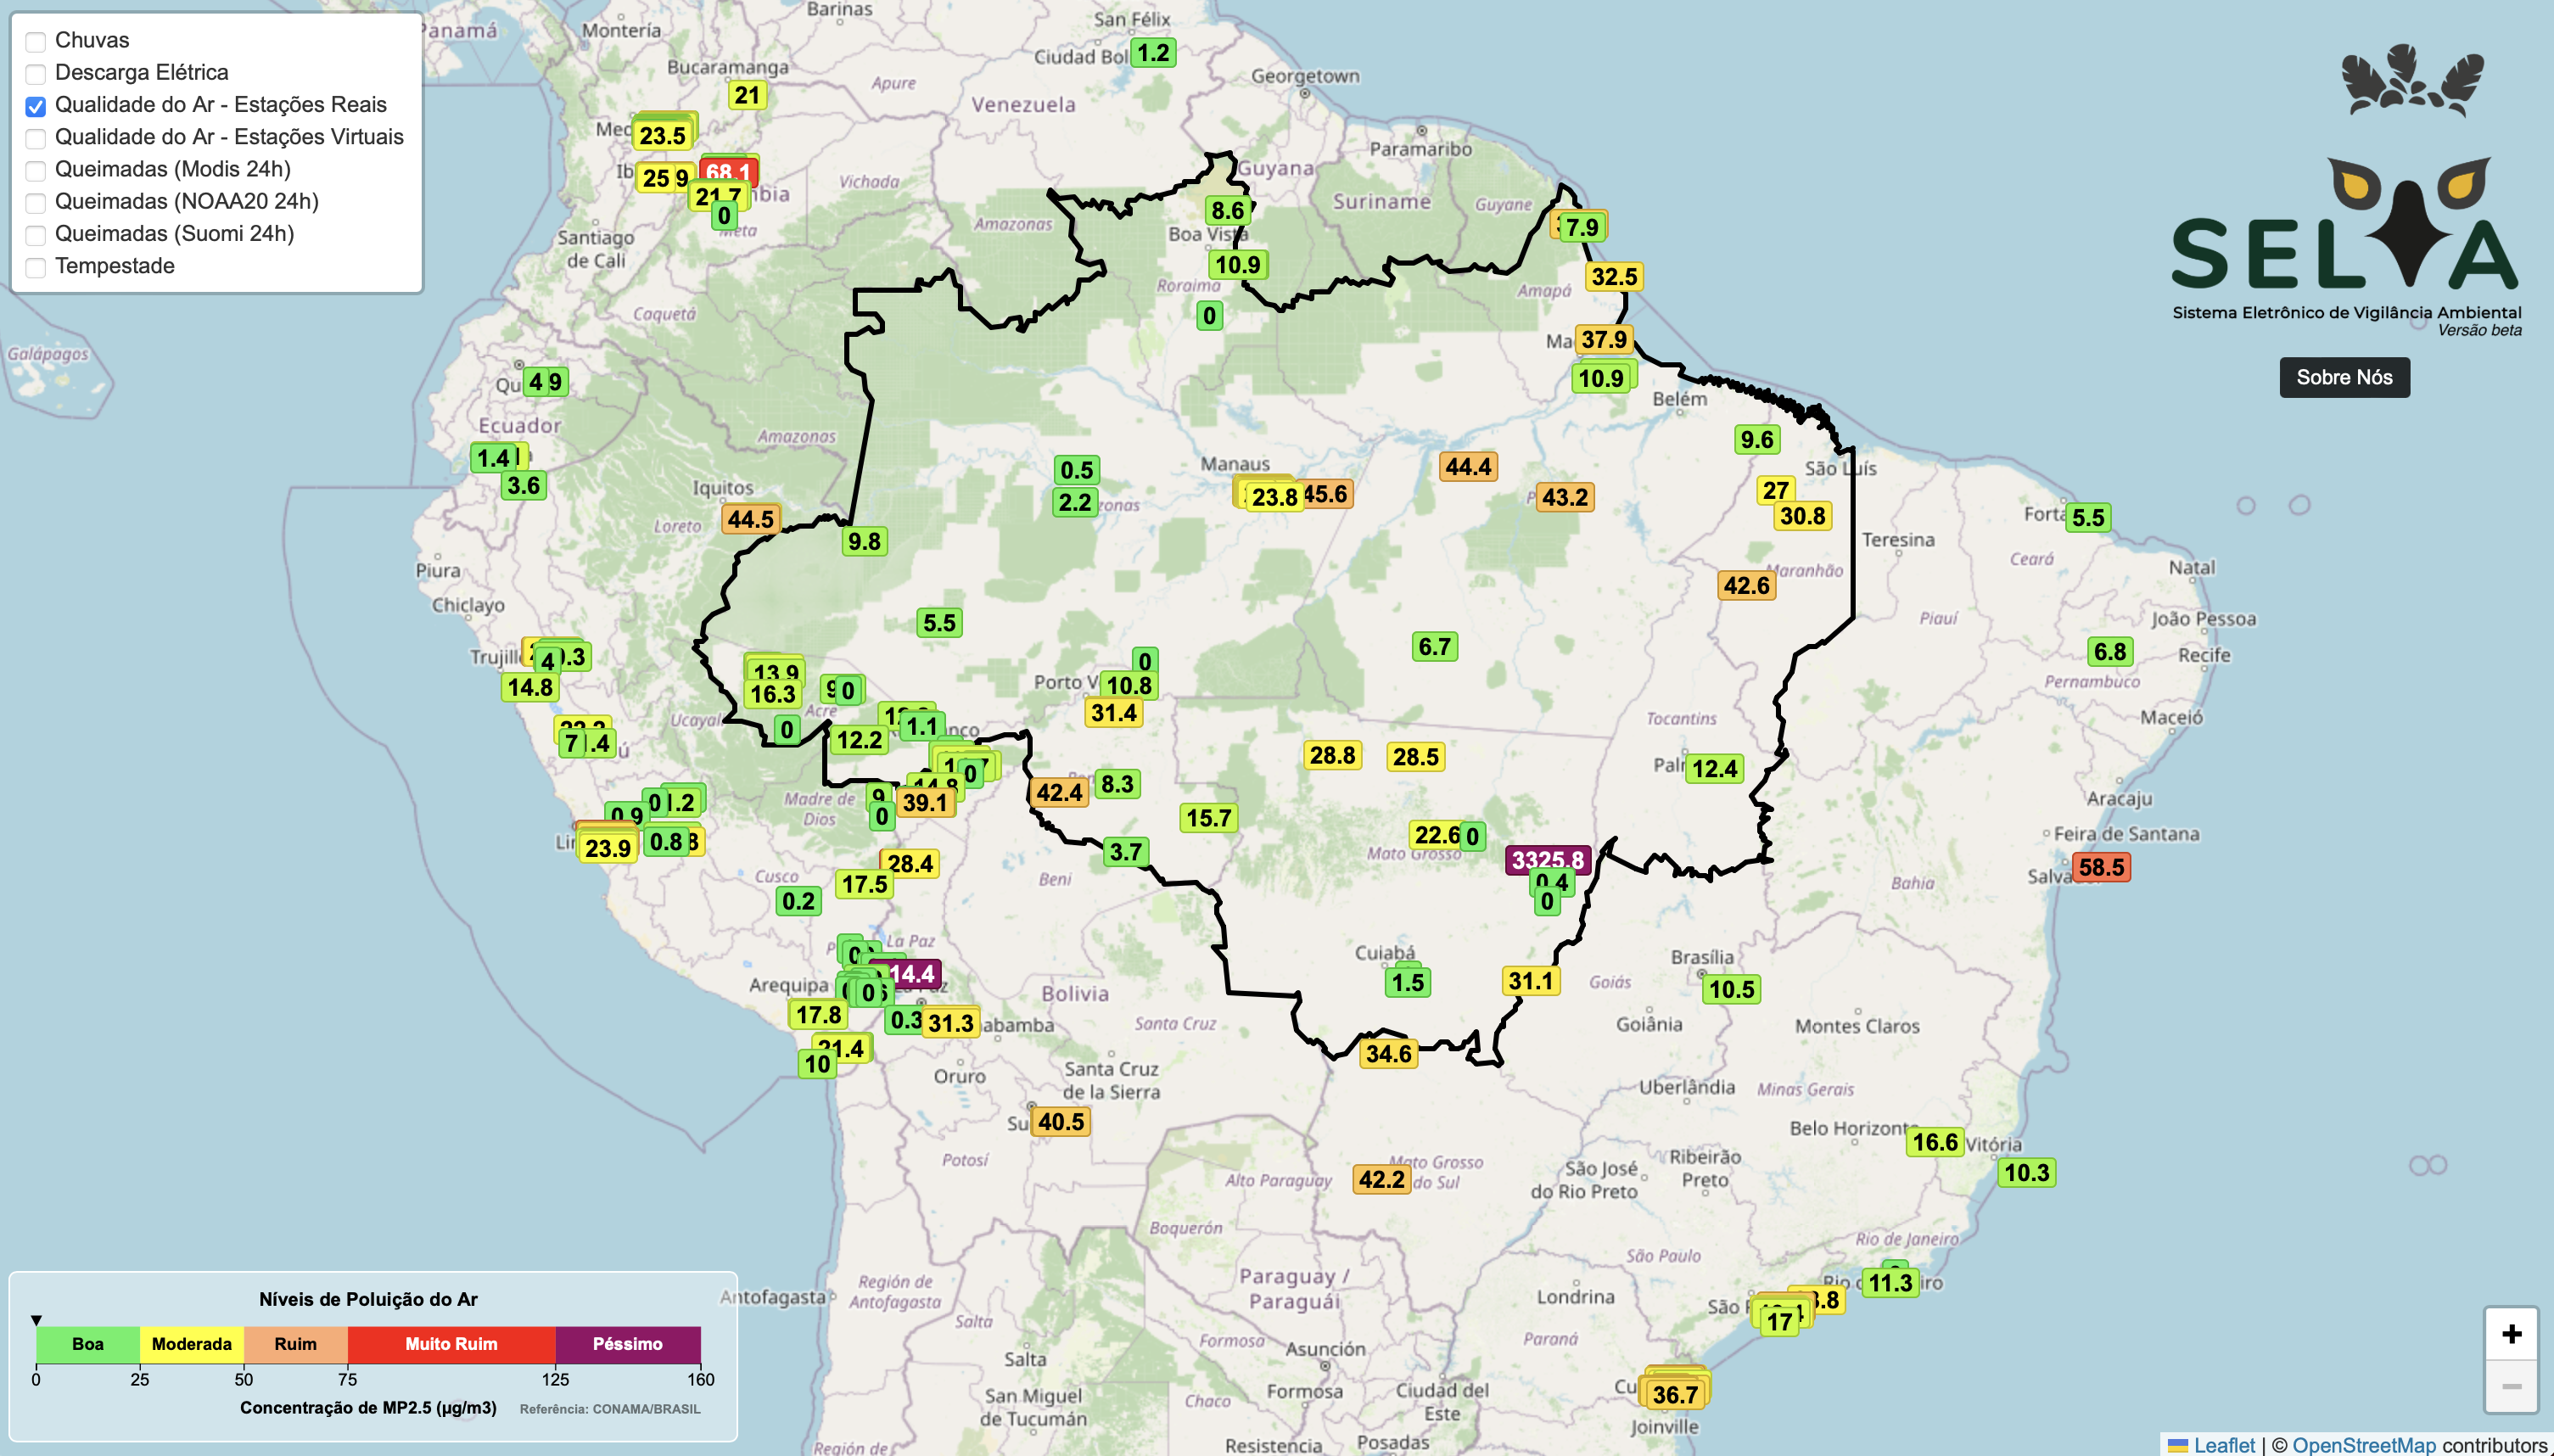
\includegraphics[width=\textwidth]{chapters/1-MONITORAMENTO/Figuras/SELVA.png}
    \label{fig:selva-purple-air}
    \fonte{\cite{Ribeiro2021}}
\end{figure}

Das iniciativas de acesso aberto, revisadas apenas a \textit{Sensor.Community} e a \textit{Smart Citizen Map} são efetivamente de código aberto. Além de disponibilizarem seus monitores para venda, ambas fornecem guias para replicação dos seus dispositivos de monitoramento e para utilização das suas \acrshort{api}s para acesso e registro de dados de monitoramento. Contudo, a documentação é apenas para replicação dos dispositivos já existentes, de acordo com um conjunto de instruções de hardware e software, e não visam facilitar o seu reaproveitamento para criação de novas topologias para aplicações diferentes. Para isso \textit{Smart Citizen} disponibiliza o \textit{Smart Citizen Kit} e \textit{Sensor.Community} disponibiliza o \textit{Sensor Kit \#1}, conforme ilustrado nas Figuras \ref{fig:smart-citizen-kit} e \ref{fig:sensor-community-kit}. Os valores dos \textit{kits} são de 119.00 USD e 50.00 EUR respectivamente.

\begin{figure}[h]
    \centering
    \caption{Os \textit{kits} de \textit{Smart Citizen} e \textit{Sensor.Community}}
    \begin{subfigure}{0.54\textwidth}
        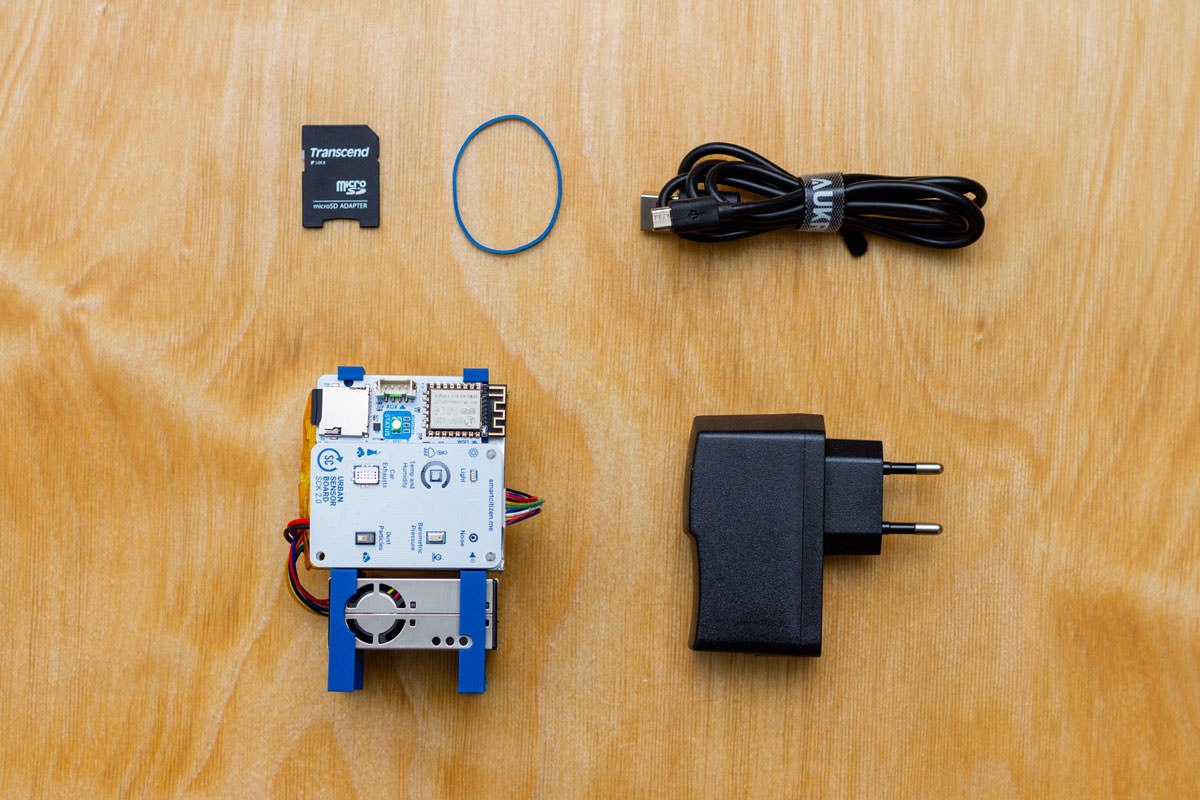
\includegraphics[width=\textwidth]{chapters/1-MONITORAMENTO/Figuras/smart-citizen-kit.jpg}
        \caption{\textit{Smart Citizen Kit} de \textit{Smart Citizen}}
        \fonte{\cite{SmartCitizen2023SmartCitizen}}
        \label{fig:smart-citizen-kit}
    \end{subfigure}
    \hfill
    \begin{subfigure}{0.45\textwidth}
        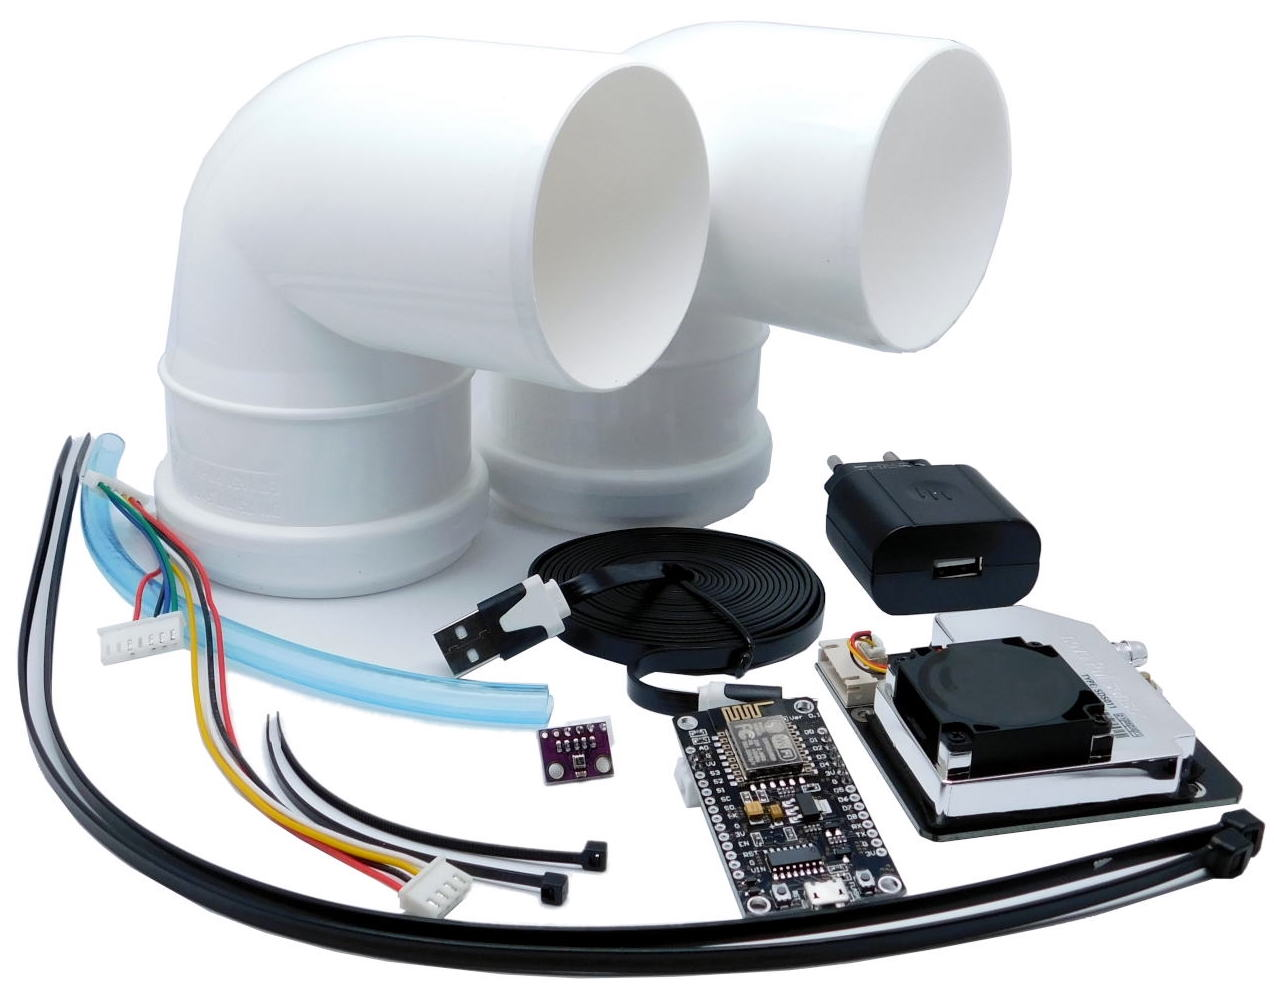
\includegraphics[width=\textwidth]{chapters/1-MONITORAMENTO/Figuras/sensor-community-kit.jpg}
        \caption{\textit{Sensor Kit \#1} de \textit{Sensor.Community}}
        \fonte{\cite{Sensor.Community2023LuftMap}}
        \label{fig:sensor-community-kit}
    \end{subfigure}
    \hfill
\end{figure}

Estes esforços tem expandido as redes de monitoramento de poluição atmosférica e incorporado as comunidades e os cidadãos no acesso a dados de qualidade do ar. Contudo, o acesso aos dispositivos ainda é limitada, especialmente nos países em desenvolvimento onde o custo do dólar costuma ser mais elevado. Como a maioria destes instrumentos são comerciais, enquadram-se na categoria de “caixa preta” e não facilitam a sua replicação. Por outro lado, as iniciativas de código e de \textit{hardware} aberto desenvolvem com foco em aplicações específicas e seguindo topologias que não visam necessariamente a modularização para reaproveitamento em outras aplicações. Isso ainda representa uma limitante dada a heterogeneidade de aplicações de monitoramento, já que sempre que uma nova aplicação surgir, novos códigos e novos \textit{hardwares} precisarão ser desenvolvidos. Dentro do contexto brasileiro, não foram encontradas iniciativas de produção de sensores de baixo custo em solo nacional.

% ----------------------------------------------------------
\subsection{Limitações do monitoramento de baixo custo da qualidade do ar}\label{subsection:low-cost-monit-limits}
% ----------------------------------------------------------

Os sensores de gases de baixo custo, como qualquer sistema de medição, possuem fontes de erro internas que são inerentes ao seu próprio funcionamento \cite{Maag2018ADeployments}. Estes erros são geralmente conhecidos e fáceis de determinar. Além desses, existem fontes de interferência externas, relacionadas às suas condições de operação, que são mais difíceis de detectar e controlar. Inclusive, sensores de um mesmo fabricante e de um mesmo lote de fabricação, podem apresentar comportamentos diferentes perante a influência de fontes externas \cite{Alphasense2013AlphasenseHUMIDITY,Castell2017CanEstimates}.

Os fabricantes normalmente definem um intervalo de medição onde os sensores apresentam melhor desempenho. O limite inferior desse intervalo é conhecido como limite de detecção, e todos os valores inferiores a ele são considerados como ruído \cite{Maag2018ADeployments}. Esse parâmetro é determinado em condições de laboratório, por isso em condições de operação não controladas, o seu valor pode sofrer alterações levando a erros nas medições. Por exemplo, em ambientes com muitas fontes de ruído electromagnético, ou um circuito de alimentação de energia pouco robusto a flutuações na tensão elétrica, podem aumentar a amplitude do ruído elétrico e, com ele, o limite de detecção dos sensores, afetando a sua resolução.

Outro tipo de erro sistemático que se manifesta internamente são os erros de \textit{offset} e de sensibilidade. Como estes erros são não aleatórios são relativamente fáceis de remover mediante calibrações de laboratório \cite{Spinelle2013ProtocolPollution}. As derivas são outra fonte interna de erros produto de alterações na sensibilidade dos sensores devido principalmente ao seu envelhecimento, que dificultam seu uso para monitoramento a longo prazo \cite{Feng2019ReviewTechnology}. As derivas podem ser eliminadas com re-calibrações periódicas. A frequência das re-calibrações depende do sensor e da concentração de poluentes a que é exposto, podendo chegar a ser quinzenal \cite{Concas2021LOW-COSTPREPRINT}.

Fatores externos ao funcionamento dos sensores também produzem interferências nas medições. A influência desses fatores, principalmente das condições ambientais, são identificados por grande parte dos autores como um dos principais desafios no tratamento das respostas dos sensores \cite{Mead2013TheNetworks,Popoola2016DevelopmentStability,Rai2017End-userMonitoring,Baron2017AmperometricReview}. Esses problemas são característicos de medições feitas em ambientes externos, em condições e ambientes reais, não controladas, ao contrário das medições tomadas em condições de laboratório sob as quais o desempenho dos sensores costuma ser muito melhor \cite{Castell2017CanEstimates}.

Variações na temperatura e na umidade do ambiente afetam a sensibilidade e o valor de linha base dos sensores \cite{Popoola2016DevelopmentStability,Pang2018TheMonitoring}. Particularmente, tem sido observado que em ambientes externos, onde os níveis de concentração costumam encontrar-se na ordem dos \gls{ppb}, as variações na temperatura e na umidade relativa alteram o valor de linha base em maior medida que a sensibilidade \cite{Popoola2016DevelopmentStability}.

Os fabricantes de sensores muitas vezes disponibilizam informações sobre a relação entre as respostas dos sensores e as variáveis ambientais, junto a modelos lineares de compensação \cite{Alphasense2013AlphasenseHUMIDITY,SPECSensors2016ApplicationPerformance}. No entanto, essas informações são obtidas a partir de testes de laboratório que simulam condições reais \cite{Spinelle2013ProtocolPollution}, sendo válidas apenas em níveis de concentração na ordem dos \gls{ppm} e em condições similares às dos testes \cite{Lewis2018Low-costApplications}. Dessa forma, as soluções para compensar os efeitos da temperatura e a umidade relativa providas pelos fabricantes resultam insuficientes para aplicações em campo \cite{Pang2018TheMonitoring}. Essas informações são especialmente limitadas para aplicações de monitoramento móvel, onde os sensores são expostos a transientes de concentração bruscos e condições ambientais variadas \cite{Delaine2019InReview}.
	
Uma solução que o fabricante Alphasense tem aplicado nos seus sensores é a incorporação de um quarto eletrodo, chamado eletrodo auxiliar, cujo sinal de saída é utilizado para compensar os efeitos de variáveis ambientais no valor de linha base do sensor \cite{Alphasense2019AlphasenseSensors}. Este eletrodo tem uma composição similar ao eletrodo de trabalho e provê um sinal de corrente de linha base que acompanha as variações do eletrodo de trabalho decorrentes das mudanças na temperatura, a umidade relativa e a pressão, podendo ser subtraída para obter a resposta do sensor ao gás \cite{Baron2017AmperometricReview}. Idealmente deveria funcionar assim, contudo, na prática tem sido demonstrado que o eletrodo auxiliar não é capaz de acompanhar as variações do eletrodo de trabalho em todo o intervalo de temperaturas de operação, e que portanto, uma simples subtração é insuficiente para gerar uma resposta confiável \cite{Wei2018ImpactMonitoring}. Cross e colaboradores também comprovaram que as correções recomendadas pelo fabricante Alphasense utilizando o eletrodo auxiliar não produzem os níveis de acurácia requeridos nas medições em ambientes externos \cite{Cross2017UseMeasurements}.
	
Tem sido reportado que variações bruscas na umidade relativa e na pressão ambiente produzem picos nas respostas dos sensores que invalidam as leituras por intervalos de tempo de até 40 minutos \cite{Alphasense2013AlphasenseHUMIDITY,Lewis2018Low-costApplications}. Igualmente ambientes com valores de umidade muito extremos ou muito poluídos podem saturar os sensores ocasionando falhas e reduzindo sua sensibilidade \cite{Alphasense2013AlphasenseHUMIDITY}.

Outros fatores que influenciam no desempenho dos sensores são as variações nos níveis de concentração do local de instalação. Os sensores eletroquímicos, por exemplo costumam ter melhor desempenho em locais onde os níveis de poluição são elevados \cite{Castell2017CanEstimates}, já que nestas condições a dinâmica senso-gás predomina sobre o efeito das variáveis interferentes \cite{Hagan2018CalibrationInstruments}. Por exemplo, Hagan e colaboradores comprovaram que o efeito da umidade relativa poderia ser ignorado ao calibrar um sensor \gls{ec} sensível a \acrshort{so2} em todo o intervalo de medição do sensor, contudo, para medições abaixo de 25 ppb, o efeito da umidade relativa mostrou-se significativa \cite{Hagan2018CalibrationInstruments}. Nuria Castell e colaboradores obtiveram coeficientes de correlação maiores com sensores instalados em locais com trânsito intenso do que nos locais com trânsito leve \cite{Castell2017CanEstimates}. Eles também constataram que o coeficiente de correlação dos sensores testados em locais com trânsito intenso caiu de forma considerável durante o período de férias, quando o trânsito pelo local foi reduzido \cite{Castell2017CanEstimates}. Por esse motivo, outro dos desafios dos monitores de baixo custo é que os instrumentos mantenham um bom desempenho independentemente dos níves de concentração encontrados no local \cite{Concas2019ACalibration}.

Outro problema comum dos sensores de baixo custo é a sensibilidade cruzada, que é a sensibilidade que os sensores têm a outros gases além do gás de interesse \cite{Maag2018ADeployments}. Por exemplo, é bem conhecido que os sensores de \acrshort{o3} são também sensíveis ao \acrshort{no2} \cite{Pang2017ElectrochemicalMonitoring,Alphasense2019AlphasenseSensors}. Outros estudos têm encontrado também sensibilidade a \acrshort{no2} em sensores de \acrshort{no} e \acrshort{so2} \cite{Lewis2016EvaluatingResearch}, assim como a \acrshort{o3} e \acrshort{co2} em sensores de \acrshort{no2} \cite{Lewis2018Low-costApplications}. Este efeito é especialmente desvantajoso em ambientes externos onde o ar é formado por uma mistura complexa de compostos gasosos. Por isso, se faz necessário assegurar que a leitura de um sensor corresponda ao gás para o qual foi projetado sem a interferência de outros compostos.

Uma forma de abordar o problema da sensibilidade cruzada é otimizando o material do eletrodo de trabalho durante a fabricação do sensor, para facilitar ou catalisar apenas as reações do gás de interesse \cite{R.Stetter2008AmperometricReview}. Igualmente, a seletividade pode ser melhorada no circuito de condicionamento, fixando o potencial de trabalho em um valor que favoreça as reações para o gás objeto de estudo \cite{R.Stetter2008AmperometricReview,Alphasense2013AlphasenseWork}. Em ambientes externos essas abordagens costumam ser insuficientes, sendo necessário utilizar arranjos de sensores nas medições e aplicar técnicas de calibração multivariadas que considerem a resposta global do arranjo \cite{Maag2018ADeployments}.

Dada a multiplicidade e complexidade dos fatores que influenciam as medições dos sensores de baixo custo, se faz necessário o estudo cuidadoso e a aplicação de técnicas de calibração que garantam níveis de precisão e confiabilidade aceitáveis para cada aplicação de monitoramento. Isso é de importância especialmente nas aplicações de monitoramento móvel, em que os sensores são expostos a transientes bruscos nas condições de operação.

Com o intuito de regulamentar o uso de monitores de baixo custo segundo a confiabilidade das suas leituras, a Diretiva Europeia para a Qualidade do Ar definiu o Objetivo da Qualidade dos Dados (\gls{dqo}) como requisito necessário para o uso destes instrumentos para fins de indicação da concentração de poluentes atmosféricos \cite{EU2008DirectiveEurope}. O \gls{dqo} representa o nível de incerteza aceitável nas medições destes instrumentos sendo de 50\% para \acrshort{mp}, 30\% para \acrshort{o3} e 25\% para \acrshort{co}, \acrshort{nox} e \acrshort{so2}. A Agência de Proteção Ambiental Norte-americana (\gls{epa}), por outro lado, sugere a avaliação dos instrumentos de monitoramento considerando cinco áreas de aplicação (Tabela \ref{tab:monitoring-areas-EPA}). Cada área tem valores de precisão, viés e completude dos dados que devem ser cumpridos para que um monitor de baixo custo possa ser utilizado em aplicações dentro dessa área \cite{Williams2014AirGuidebook}. Numa direção um pouco diferente dos dois órgãos anteriores, em um estudo mais recente conduzido por Lidia Morawska, foi proposto que, dado o amplo leque de aplicações de monitoramento, os requisitos de desempenho dos monitores de baixo custo fossem definidos de acordo com cada aplicação prescindindo assim de métricas padrões \cite{Morawska2018ApplicationsGone}. Esta última abordagem, contudo, exige um conhecimento profundo da aplicação e dos requerimentos de desempenho associados \cite{Morawska2018ApplicationsGone}.

\begin{table}[t]
    \caption{Requerimentos de desempenho dos instrumentos de monitoramento da qualidade do ar segundo área de aplicação}
    \begin{tabular}{ m{0.35\textwidth} m{0.3\textwidth} m{0.10\textwidth} m{0.15\textwidth}}
        \hline
        Área de aplicação & Poluentes & Erro & Completude dos dados \\ [0.5ex] 
        \hline
        Educação e Informação & Todos & < 50\% & $\geq$ 50\% \\ [0.5ex]
        \hline
        Identificação e Caracterização de \textit{Hotspots}\footnotemark & Todos & < 30\% & $\geq$ 75\% \\ [0.5ex]
        \hline
        Monitoramento Complementar & Todos os regulados pelo \gls{conama} e os \acrshort{voc} & < 20\% & $\geq$ 80\% \\ [0.5ex]
        \hline
        Exposição pessoal & Todos & < 30\% & $\geq$ 80\% \\ [0.5ex]
        \hline
        Monitoramento de referência & \acrshort{o3} \newline \acrshort{co}, \acrshort{so2} \newline \acrshort{no2} \newline \acrshort{mp} & < 7\% \newline < 10\% \newline < 15\% \newline < 10\% & $\geq$ 75\% \\ [0.5ex]
        \hline
    \end{tabular}
    \label{tab:monitoring-areas-EPA}
    \fonte{\cite{Williams2014AirGuidebook}}
\end{table}
\footnotetext{Pontos de elevada concentração de determinado poluente}